In this section, we are going to show the numerical results for computing the Casimir energy between two perfectly conducting objects, which are spheres, 
menger sponges, ice crystals and ellipsoids. The reference value of the Casimir energy is computed by the Richardson extrapolation method which is often used 
for obtaining the higher-order estimate at zero grid spacing. Denote $\mathcal{E}_{\text{fine}}$ and $\mathcal{E}_{\text{coarse}}$ as the Casimir energy 
numerically computed from the formula \eqref{KSSF and CasE} by setting the grid size $h$ as $h_{\text{fine}}$ and $h_{\text{coarse}}$ 
($h_{\text{fine}}<h_{\text{coarse}}$), separately. Then, the high-accuracy result $\mathcal{E}_{\text{exact}}$ can be generated from the following formula:
\begin{align}\label{Richardson extrapolation}
    \mathcal{E}_{\text{exact}} \approx \mathcal{E}_{\text{fine}} + \frac{h_{\text{coarse}}^{2}\mathcal{E}_{\text{fine}} - h_{\text{fine}}^{2}\mathcal{E}_{\text{coarse}}}{h_{\text{coarse}}^{2} - h_{\text{fine}}^{2}}.
\end{align}
In addition, the asymptotic series of the Casimir energy are also available in two spheres' case and the series can be found in \cite{emig2008casimir} 
for both equal and unequal radii's cases. 

\subsection{Two spheres case}
\begin{figure}[H]
    \hspace*{3cm}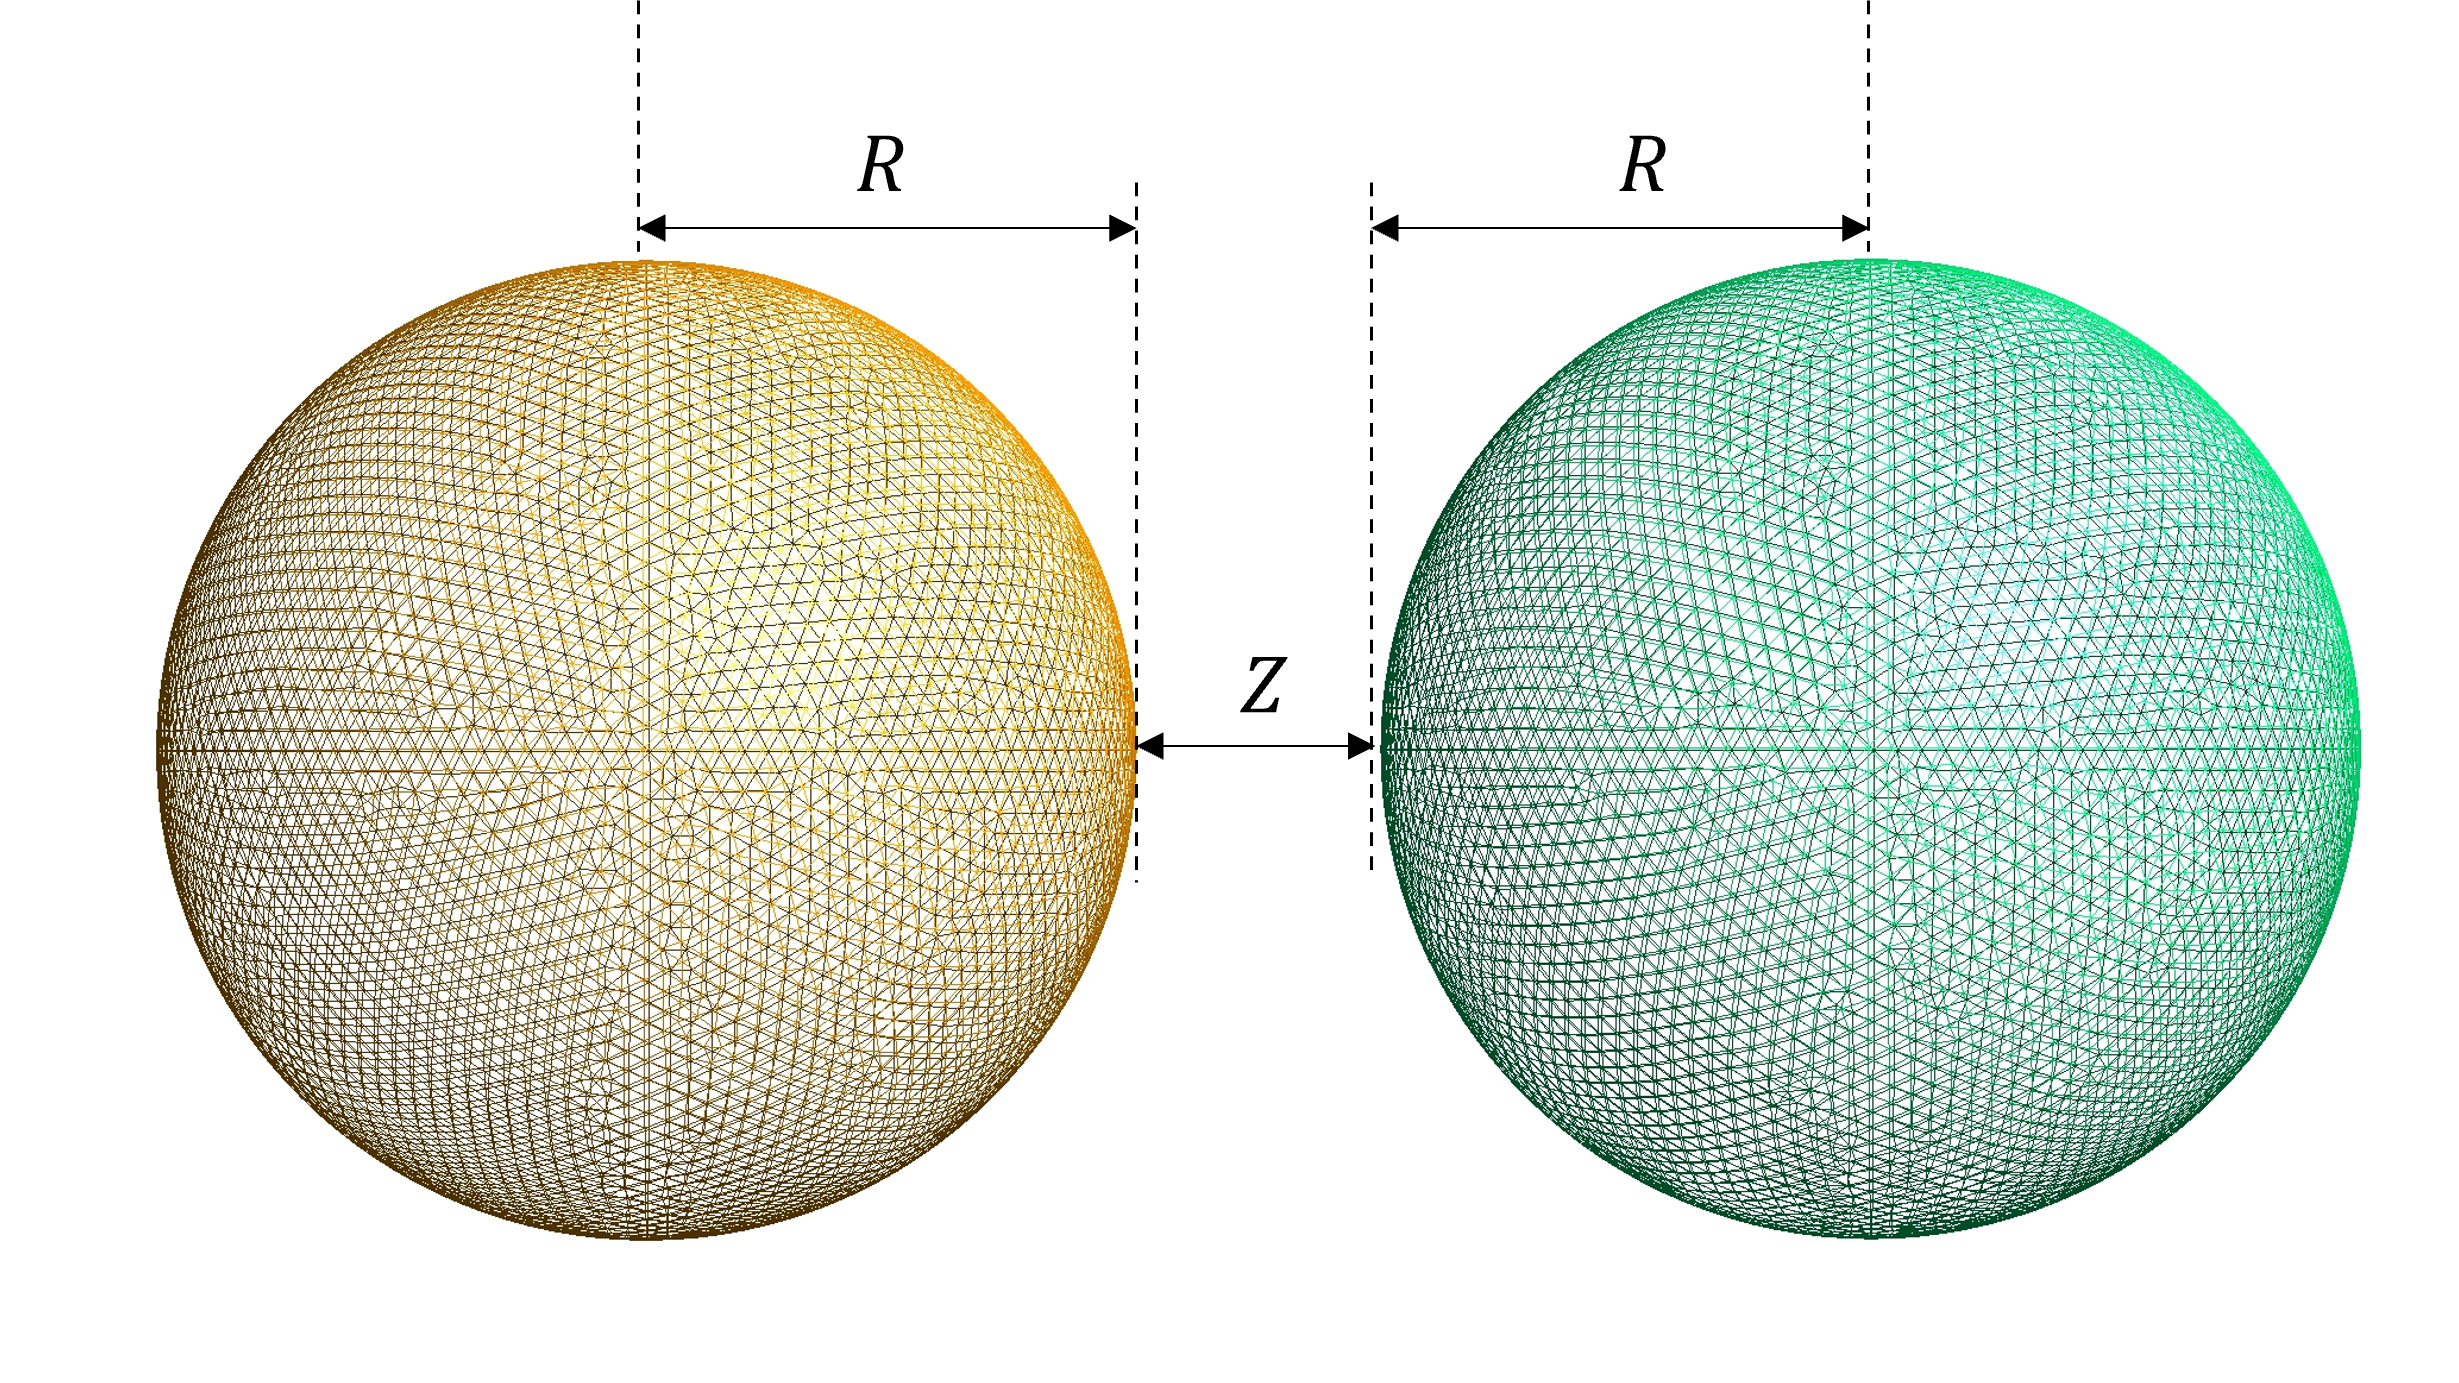
\includegraphics[scale = 0.6]{figures/Grid_two_spheres_dist.png}
    \caption{Two spheres with equal radii: $R$ represents the radius of the spheres and $Z$ is the distance between them.}
    \label{Two spheres with equal radii}
\end{figure}

Consider two perfectly conducting spheres with equal radii, which are shown in the Figure \ref{Two spheres with equal radii}. Inside the figure, $R$ is the radius 
of the spheres and the distance between them is denoted as $Z$. We begin with estimating the Casimir energy between two spheres with radius $R = 1$ at the 
distance of $Z$ via the formula \eqref{KSSF and CasE} in two different refinement levels: $h_{\text{fine}} = 0.05$ and $h_{\text{coarse}} = 0.1$ and the 
distance $Z$ between them is ranging from 0.5 to 3.0. Afterwards, the extrapolation result can be obtained by substituting these Casimir energy estimates into 
the formula \eqref{Richardson extrapolation}. This result would be regarded as the exact value of the Casimir energy and can be used to compare with the 
estimates derived from the asymptotic series introduced below. 

According to \cite{emig2008casimir}, the Casimir energy between two spheres (with equal radii $R$) at asymptotically 
large separations can be obtained as a series in terms of the ratio of centre distance $L$ ($L = 2R + Z$) to sphere radius $R$:
\begin{align}\label{Asymptotic equal radii}
   \mathcal{E} = -\frac{\hbar c}{\pi}\frac{1}{L}\sum_{n=0}^{\infty}b_{n}\left(\frac{R}{L}\right)^{n+2},
\end{align}
where the first six coefficients are 
$b_{0} = -1/4$, $b_{1} = -1/4$,  $b_{2} = -77/48$,  $b_{3} = -25/16$,  $b_{4} = -29837/2880$, $b_{5} = -6491/1152$. Figure 
\ref{Casimir energy between spheres with equal radii} shows the comparison between the Casimir energy computed from asymptotic series 
\eqref{Asymptotic equal radii} and the exact value evaluated through {Richardson extrapolation}. Here, we observe that the asymptotic value gradually 
approaches to the exact value as the distance $Z$ increases since the asymptotic expansion \eqref{Asymptotic equal radii} only works when the distance 
between two spheres is asymptotically large.

\begin{figure}[H]
    \includegraphics[scale = 0.7]{figures/Spheres_equal_CasE.pdf}
    \caption[Caption for LOF]{Normalized Casimir energy\protect\footnotemark in two spheres with equal radii's case. The radius is $R = 1$ and the distance $Z$ 
    ranges from 0.5 to 3.0. The exact value of the (normalized) Casimir energy has been written beside the data point, which is round up to 4 significant digits.}
    \label{Casimir energy between spheres with equal radii}
\end{figure}
\footnotetext{The normalized Casimir energy is $\mathcal{E}/\hbar c$, for $\mathcal{E}$ defined in \eqref{KSSF and CasE}.}

Afterwards, in order to test the performance of the two efficient methods introduced in Section \ref{Krylov subspace for generalized eigenvalue problem}, we
would use them to evaluate the Casimir energy between two spheres described above. For the inverse-free Krylov subspace method, the dimension of the Krylov subspace is set as $m = 20$ and 50 and the 
number of approximated smallest (or largest) eigenvalues is $p = 10$ and 25, respectively. For the standard Arnoldi method, the dimension of the 
Krylov subspace is also set as $m = 20$ and 50. 

Figure \ref{equal_radii_rel_dist} shows the relative distance between the estimates computed through inverse-free Krylov subspace method 
(dashed/solid green triangles), standard Arnoldi method (dashed/solid blue circles), asymptotic series (solid black square) and the exact values.
Here, we can easily see that the inverse-free Krylov subspace method behaves better than the standard Arnoldi method no matter when the dimension $m$ is 
20 or 50 and as we increase the Krylov subspace dimension, the relative error decreases.

In addition, it can be noticed that when the distance $Z$ between the spheres increases, the relative error 
for both methods goes down. The reason appears to be that the cross interaction between them becomes weaker as the spheres are getting away from each other. 
This leads the compact perturbation $\tilde{\mathsf{V}}_{k}$ to become close to $\mathsf{V}_{k}$, which reduces the number of the eigenvalues that mainly 
contribute on the log determinant of $\mathsf{V}_{k}\tilde{\mathsf{V}}_{k}^{-1}$. Therefore, if we keep setting the same dimension of Krylov subspace 
for the spheres are at a large distance, we would have a better approximation on the Casimir energy.


\begin{figure}[H]
    \includegraphics[scale = 0.7]{figures/relative_distance_equal_radii.pdf}
    \caption{Relative distance between the reference value (computed by Richardson extrapolation) with the asymptotic series (solid black square)  
    and the estimates evaluated from the standard Arnoldi method (dashed/solid blue circles) and inverse-free Krylov subspace method (dashed/solid green triangles) 
    by setting the dimension of the Krylov subspace as $m = 20$ and 50 and for the inverse-free
    Krylov subspace method, the number of the approximated smallest (or largest) eigenvalues is set as $p = 10$ and 25, respectively.}
    \label{equal_radii_rel_dist}
\end{figure}
 
%================================================================================================================
\begin{figure}[H]
    \hspace*{2cm}\includegraphics[scale = 0.6]{figures/Grid_two_spheres_unequal_radii.png}
    \caption{Two spheres with unequal radii: $R_{1}$ and $R_{2}$ represent the radius of the spheres and $Z$ is the distance between them.}
    \label{Two spheres with unequal radii}
\end{figure}

When the perfectly conducting spheres have different radii $R_{1}$, $R_{2}$ (see Figure \ref{Two spheres with unequal radii}) and the centre distance is denoted as
$L = R_{1} + R_{2} + Z$, the asymptotic expansion of the Casimir energy at asymptotically large distance can be written as:
\begin{align}\label{Asymptotic unequal radii}
    \mathcal{E} = -\frac{\hbar c}{\pi}\frac{1}{L}\sum_{n=0}^{\infty}\tilde{b}_{n}(\eta)\left(\frac{R_{1}}{L}\right)^{n+2},
\end{align}
where the coefficients $\{\tilde{b}_{n}\}$ depend on the parameter $\eta = R_{2}/R_{1}$ and the first six coefficients are
\begin{align*}
    \tilde{b}_{0} &= -\frac{\eta}{4}, \ \ \ \ \ \tilde{b}_{1} = -\frac{\eta + \eta^{2}}{8}, \ \ \ \ \  \tilde{b}_{2} = -\frac{34(\eta+\eta^{3})+ 9\eta^{2}}{48}, \ \ \ \ \ \tilde{b}_{3} = -\frac{2(\eta+\eta^{4}) + 23(\eta^{2} + \eta^{3})}{32}, \\ 
    \tilde{b}_{4} &= -\frac{8352(\eta + \eta^{5})+ 1995(\eta^{2} + \eta^{4}) + 38980\eta^{3}}{5760}, \ \ \ \ \ \tilde{b}_{5} = -\frac{-1344(\eta+\eta^{6}) + 5478(\eta^{2} + \eta^{5})+2357(\eta^{3} + \eta^{4})}{2304}.
\end{align*}

In the following experiment, the radii of the spheres shown in Figure \ref{Two spheres with unequal radii} are set as $R_{1} = 0.5$ and $ R_{2} = 1$. 
As in the previous example, the exact value of the Casimir energy is computed through the Richardson extrapolation formula \eqref{Richardson extrapolation}, 
where the coarse and fine grid size are $h_{\text{coarse}} = 0.1$ and $h_{\text{fine}} = 0.05$, separately. In this case, the asymptotic value of the Casimir 
energy was estimated by the series \eqref{Asymptotic unequal radii} and the comparison between the exact value and asymptotic one is shown in Figure 
\ref{Casimir energy between spheres with unequal radii}. Again we see that when the distance between two spheres decreases, the asymptotic value gets 
close to the exact one and the reason for this is clearly stated in the above equal radii's case.
\begin{figure}[H]
    \includegraphics[scale = 0.7]{figures/Spheres_unequal_CasE.pdf}
    \caption{Normalized Casimir energy in two spheres with unequal radii's case. The radius is $R = 1$ and the distance $Z$ 
    ranges from 0.5 to 3.0. The exact value of the (normalized) Casimir energy has been written 
    beside the data point, which is round up to 4 significant digits.}
    \label{Casimir energy between spheres with unequal radii}
\end{figure}

By keeping all the experimental settings being the same with the equal radii's case, the numerical experiments on testing the performance of the inverse-free and 
standard Arnoldi methods have been done in the unequal radii's case and the results are shown in Figure \ref{unequal_radii_rel_dist}, from which we observe that 
the results between these two efficient methods have no big difference except the standard Arnoldi case when the dimension $m = 20$.  Compared with the previous
case, it is supposed to be due to the smaller scatterer, leading to the smaller number of eigenvalues that makes significant influence on the log determinant.

\begin{figure}[H]
    \includegraphics[scale = 0.7]{figures/relative_distance_unequal_radii.pdf}
    \caption{Relative distance between the reference value (computed by Richardson extrapolation) with the asymptotic series (solid black square)  
    and the estimates evaluated from the standard Arnoldi method (dashed/solid blue circles) and inverse-free Krylov subspace method (dashed/solid green triangles) 
    by setting the dimension of the Krylov subspace as $m = 20$ and 50 and for the inverse-free
    Krylov subspace method, the number of the approximated smallest (or largest) eigenvalues is set as $p = 10$ and 25, respectively.}
    \label{unequal_radii_rel_dist}
\end{figure}

\subsection{Realistic objects case}
In this part, the Casimir energy between the objects with special shapes such as the menger sponges, ice crystals and ellipsoids will be computed and 
the values labelled in the following figures are always round up to 4 significant digits. 

Figure \ref{Menger sponges} plots the menger sponges in different levels $(0, 1 $ and $ 2)$ and the length of these sponges is always 1. Afterwards, the Casimir 
energy between two menger sponges in the same level are plotted in Table \ref{Normalized Casimir energy in two menger sponges' case}. By comparing the data 
point in these subfigures, it is easy to find that the Casimir energy decreases as the number of the iteration increases since the cross-sectional 
area gets smaller.

\begin{figure}[H]
    \centering
    \subfloat[Level 0]{{\includegraphics[width=0.4\textwidth]{figures/merger_sponge_level0.jpg} }}
    \qquad
    \subfloat[Level 1]{{\includegraphics[width=0.4\textwidth]{figures/merger_sponge_level1.jpg} }}
    \qquad
    \subfloat[Level 2]{{\includegraphics[width=0.4\textwidth]{figures/merger_sponge_level2.jpg} }}
    \caption{Menger sponges in different levels. The length of each sponge is 1.}
    \label{Menger sponges}
\end{figure}

\begin{table}[H]
    \centering
    \begin{tabular}{ |p{2cm}||p{2cm}|p{2cm}|p{2cm}|  }
        \hline
        \multicolumn{4}{|c|}{Normalized Casimir energy in two menger sponges' case} \\
        \hline
        Distance & Level 0 & Level 1 & Level 2\\
        \hline
        0.5   & 0.08352    & 0.080737    & 0.07979\\
        0.75  & 0.02735    & 0.02686     & 0.02669\\
        1.0   & 0.01305    & 0.1288      & 0.01282\\
        1.25  & 0.007358   & 0.007281    & 0.007253\\
        1.5   & 0.004607   & 0.004568    & 0.004551\\
        1.75  & 0.003099   & 0.003076    & 0.0030658\\
        2.0   & 0.002196   & 0.002181    & 0.002174\\
        2.25  & 0.001619   & 0.001609    & 0.001604\\
        2.5   & 0.001231   & 0.001224    & 0.00122\\
        2.75  & 0.0009599  & 0.0009546   & 0.000952\\
        3.0   & 0.0007644  & 0.0007603   & 0.0007583\\
        \hline
       \end{tabular}
       \caption{\label{Normalized Casimir energy in two menger sponges' case} Normalized Casimir energy in two menger sponges' case}
    \end{table}

%==========================================================================================
In the next example, the scatterers are ice crystals with different number of branches ranging from 2 to 6 (see Figure \ref{Ice crystals with different number of branches}).
By Figure \ref{Normalized Casimir energy in ice crystals' case}, when the number of branches increases from 2 to 4, the Casimir energy increases as expected. But 
when the branches number added up to 5 and 6, the Casimir energy is much smaller since the main cross-sectional part cannot be as close as the 
2, 3, 4-branches cases. 

\begin{figure}[H]
    \begin{subfigure}{0.3\linewidth}
        \centering
        \includegraphics[scale = 0.4]{figures/2branches}
        \caption{Two branches}
        \end{subfigure}
        \begin{subfigure}{0.3\linewidth}
            \centering
            \includegraphics[scale = 0.4]{figures/3branches}
            \caption{Three branches}
            \end{subfigure}
            \begin{subfigure}{0.3\linewidth}
                \centering
                \includegraphics[scale = 0.38]{figures/4branches}
                \caption{Four branches}
                \end{subfigure}\\[1ex]
    \begin{subfigure}{.5\linewidth}
    \centering
    \hspace*{-1cm}\includegraphics[scale = 0.4]{figures/5branches}
    \caption{Five branches}
    \end{subfigure}%
    \begin{subfigure}{.5\linewidth}
    \centering
    \includegraphics[scale = 0.4]{figures/6branches}
    \caption{Six branches}
    \end{subfigure}
    \caption{Ice crystals with different number of branches}
    \label{Ice crystals with different number of branches}
    \end{figure}

    \begin{figure}[H]
        \centering
        \hspace*{-1cm}\includegraphics[scale = 0.5]{figures/CasE_ice_crystals.pdf}
        \caption{Normalized Casimir energy in ice crystals' case. To make the figure keep clear, only the 4-branches and 6-branches's case data points 
        are labelled in the figure. Other cases' information are listed in Table \ref{Normalized Casimir energy in ice crystals' case table}. }
        \label{Normalized Casimir energy in ice crystals' case}
    \end{figure}

    \begin{table}[H]
        \centering
        \begin{tabular}{ |p{2cm}||p{2cm}|p{2cm}|p{2cm}|p{2cm}|p{2cm}|  }
            \hline
            \multicolumn{6}{|c|}{Normalized Casimir energy in two menger sponges' case} \\
            \hline
            Distance & 2-branches & 3-branches & 4-branches & 5-branches & 6-branches\\
            \hline
            0.5   & 0.04085    & 0.05963    & 0.07814  & 0.02131    & 0.01123\\
            0.75  & 0.01498    & 0.02182    & 0.02851  & 0.01013    & 0.005016\\
            1.0   & 0.007403   & 0.010803   & 0.01412  & 0.005834    & 0.002966\\
            1.25  & 0.004242   & 0.006199   & 0.008113 & 0.003730    & 0.001985\\
            1.5   & 0.002672   & 0.003905   & 0.005118 & 0.002553    & 0.001427\\
            1.75  & 0.001268   & 0.002624   & 0.003443 & 0.001835    & 0.001075\\
            2.0   & 0.002196   & 0.001850   & 0.002428 & 0.001369   & 0.0008363\\
            2.25  & 0.0009290  & 0.001353   & 0.001777 & 0.001051    & 0.0006670\\
            2.5   & 0.0007010  & 0.001019   & 0.001339 & 0.0008261    & 0.0005424\\
            2.75  & 0.0005420  & 0.0007867  & 0.001034 & 0.0006621    & 0.0004482\\
            3.0   & 0.0004277  & 0.0006198  & 0.0008147 & 0.0005394    & 0.0003754\\
            \hline
           \end{tabular}
           \caption{\label{Normalized Casimir energy in ice crystals' case table} Normalized Casimir energy in two ice crystals' case}
        \end{table}
%==================================================================================================
It is not hard to imagine that the Casimir energy would be different after the scatterers rotate while keeping the distance between them unchanged. Therefore, 
in the last example, we would see how the Casimir energy between two identical ellipsoids changes as one of the ellipsoids rotates.

In Figure \ref{Without rotation}, the above ellipsoid is centering at $(0,0,0)$ and 
the points $(0.5, 0, 0), (0, 1, 0)$ and $(0, 0, 0.5)$ are located on this surface and if the distance between these two ellipsoids is denoted as $Z$, then the below one
is centering at $(0, 0, -(0.5+0.5+Z))$ and the points $(0.5, 0, -(0.5+0.5+Z)), (0, 1, -(0.5+0.5+Z))$ and $(0, 0, 0.5-(0.5+0.5+Z))$ are on it. Without rotation, 
the Casimir energy between them with different distance $Z$ is plotted in Figure \ref{Casimir energy between two ellipsoids with different distances}.

To explore how the rotation affects the change of the Casimir energy, one can always keep one ellipsoid fixed and rotate the other one. The Figure 
\ref{Rotation around z-axis} and \ref{Rotation around x-axis} describe the case when one of the ellipsoids rotates around $z-$ and $x-$axis, respectively.
From the Figure \ref{Casimir energy when one of the ellipsoids rotates}, the Casimir energy changes periodically since we rotate one ellipsoid around 
$z-$ or $x-$ axis by 360 degrees. 


\begin{figure}[H]
    \begin{subfigure}{\linewidth}
        \centering
        \includegraphics[scale = 0.4]{figures/two_ellipsoids}
        \caption{Without rotation}
        \label{Without rotation}
        \end{subfigure}\\[1ex]
    \begin{subfigure}{.5\linewidth}
    \centering
    \includegraphics[scale = 0.4]{figures/Ellipsoid_z_axis}
    \caption{Rotation around z-axis}
    \label{Rotation around z-axis}
    \end{subfigure}%
    \begin{subfigure}{.5\linewidth}
    \centering
    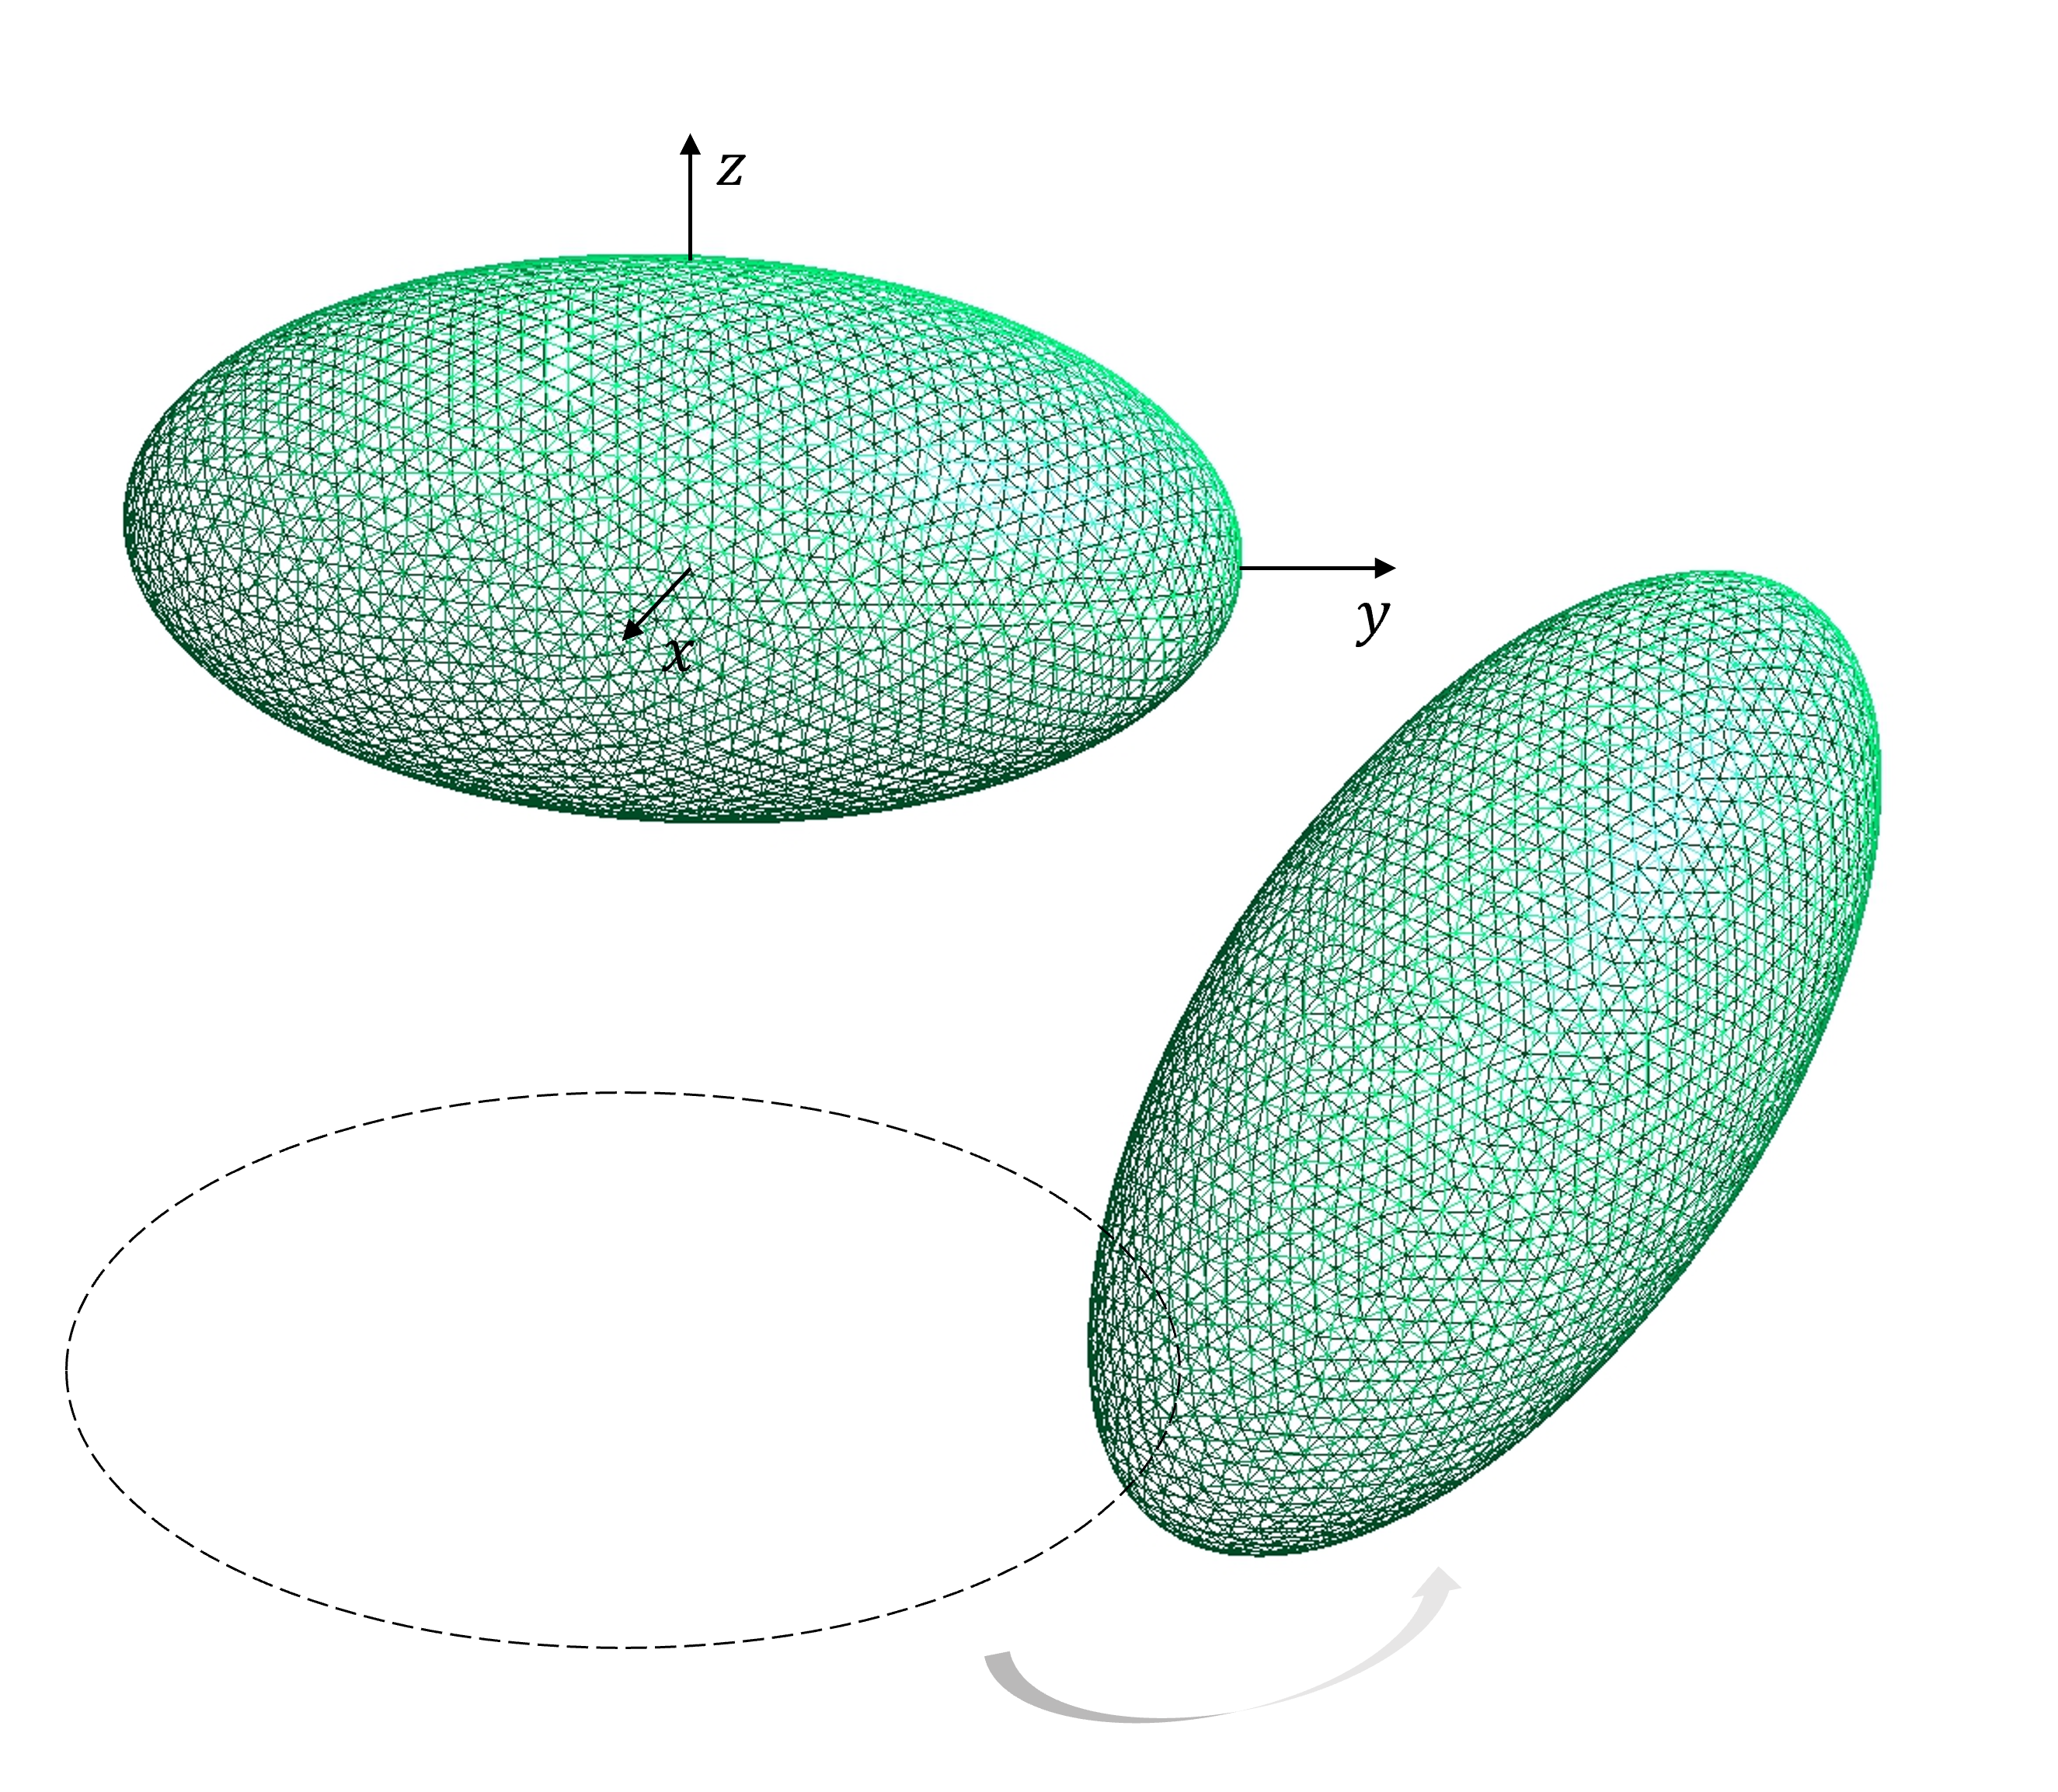
\includegraphics[scale = 0.4]{figures/Ellipsoid_x_axis}
    \caption{Rotation around x-axis}
    \label{Rotation around x-axis}
    \end{subfigure}
    \caption{Two ellipsoids with or without rotation}
    \label{Two ellipsoids}
    \end{figure}

    \begin{figure}[H]
        \begin{subfigure}{\linewidth}
            \centering
            \includegraphics[scale = 0.5]{figures/CasE_ellipsoids.pdf}
            \caption{Casimir energy between two ellipsoids with different distances}
            \label{Casimir energy between two ellipsoids with different distances}
            \end{subfigure}\\[1ex]
    
        \begin{subfigure}{\linewidth}
        \centering
        \hspace*{-1cm}\includegraphics[scale = 0.5]{figures/CasE_ellipsoids_with_rotation.pdf}
        \caption{Casimir energy when one of the ellipsoids rotates}
        \label{Casimir energy when one of the ellipsoids rotates}
        \end{subfigure}
        \caption{The dependence of the Casimir energy and rotation angle of one of the ellipsoids.} 
        \end{figure}

        \begin{figure}[H]
            \begin{subfigure}{\linewidth}
                \centering
                \includegraphics[scale = 0.4]{figures/4_ellip}
                \caption{No rotation}
                \label{No rotation 4}
                \end{subfigure}\\[1ex]
            \begin{subfigure}{.5\linewidth}
            \centering
            \includegraphics[scale = 0.4]{figures/4_ellip_in}
            \caption{Rotation inwards}
            \label{Rotation inwards 4}
            \end{subfigure}%
            \begin{subfigure}{.5\linewidth}
            \centering
            \includegraphics[scale = 0.4]{figures/4_ellip_out}
            \caption{Rotation outwards}
            \label{Rotation outwards 4}
            \end{subfigure}
            \caption{Four ellipsoids with or without rotations}
            \label{Four ellipsoids with or without rotations}
            \end{figure}

            \begin{figure}[H]
                \includegraphics[scale = 0.7]{figures/CasE_4_ellip.pdf}
                \caption{Four ellipsoids}
                \label{Four ellipsoids}
            \end{figure}


            \begin{figure}[H]
                \begin{subfigure}{\linewidth}
                    \centering
                    \includegraphics[scale = 0.4]{figures/6_ellip}
                    \caption{No rotation}
                    \label{No rotation 6}
                    \end{subfigure}\\[1ex]
                \begin{subfigure}{.5\linewidth}
                \centering
                \includegraphics[scale = 0.4]{figures/6_ellip_in}
                \caption{Rotation inwards}
                \label{Rotation}
                \end{subfigure}%
                \begin{subfigure}{.5\linewidth}
                \centering
                \includegraphics[scale = 0.4]{figures/6_ellip_out}
                \caption{Rotation outwards}
                \label{Rotation outwards 6}
                \end{subfigure}
                \caption{Six ellipsoids with or without rotations}
                \label{Six ellipsoids with or without rotations}
                \end{figure}
            
                \begin{figure}[H]
                    \includegraphics[scale = 0.7]{figures/CasE_6_ellip.pdf}
                    \caption{Six ellipsoids}
                    \label{Six ellipsoids}
                \end{figure}